\documentclass[a4paper,12pt]{article} 

%%% Работа с русским языком
\usepackage{cmap}                           % поиск в PDF
\usepackage{mathtext} 			 	       % русские буквы в формулах
\usepackage[T2A]{fontenc}               % кодировка
\usepackage[utf8]{inputenc}              % кодировка исходного текста
\usepackage[english,russian]{babel}  % локализация и переносы

%Матеша
\usepackage{amsmath,amsfonts,amssymb,amsthm,mathtools} % AMS
\usepackage{icomma} % "Умная" запятая

%\mathtoolsset{showonlyrefs=true} % Показывать номера только у тех формул, на которые есть \eqref{} в тексте.

%% Шрифты
\usepackage{euscript}	 % Шрифт Евклид
\usepackage{mathrsfs} % Красивый матшрифт

%% Свои команды
\DeclareMathOperator{\sgn}{\mathop{sgn}}

%% Перенос знаков в формулах (по Львовскому)
\newcommand*{\hm}[1]{#1\nobreak\discretionary{}
{\hbox{$\mathsurround=0pt #1$}}{}}

%%% Заголовок
\author{Злобина Вера}
\title{Лабораторная работа 1.2.2

Экспериментальная проверка закона вращательного движения на крестообразном маятнике}

\begin{document} 	
	
\maketitle

\newpage

Основное уравнение вращательного движения тела вокруг закреплённой оси:
\begin{equation}\label{1}
I \ddot{\varphi} = M, 
\end{equation}
где $\ddot{\varphi} \equiv \dot{\omega} \equiv \beta$ -- угловое ускорение ($\omega$  -- угловая скорость), $I$ -- полный момент инерции тела относительно оси вращения, $M$ -- суммарный момент внешних сил относительно этой оси.

\subparagraph*{Цель работы:} экспериментально проверить уравнение \eqref{1}, получив зависимость углового ускорения от момента инерции и момента прикладываемых к системе сил, а также проанализировать влияние сил трения, действующих в оси вращения.
\subparagraph*{Экспериментальная установка:} для экспериментального исследования закона вращательного движения \eqref{1} в работе используется крестообразный «маятник» ,  устройство которого изображено на рис. \ref{fig:image}. Маятник состоит из четырёх тонких стержней радиуса $a$, укреплённых на втулке под прямым углом друг к другу. Втулка и два шкива различных радуисов  ($r_1$ и $r_2$) насажены на общую ось. Ось закреплена в подшипниках, так что вся система может свободно вращаться вокруг горизонтальной оси. Момент инерции  $I$ маятника можно изменять, передвигая грузы $m_i (i = 1, \dots, 4)$ вдоль стержней и меняя $R_i$. На один из шкивов маятника навита тонкая нить. Привязанная к ней лёгкая платформа известной массы $m_п$ служит для размещения перегрузков $m_г$. 

Установка оснащена датчиком, позволяющим фиксировать моменты времени прохождения концов стержней через него. Данные с датчика передаются на компьютер для последующей обработки и получения зависимостей угла поворота $\varphi(t)$, угловой скорости $\omega \equiv \dot{\varphi}$ и углового ускорения маятника $\beta \equiv \ddot{\varphi}$ от времени, а также углового ускорения от угловой скорости $\beta(\omega)$.

\begin{figure}[h]
	\center{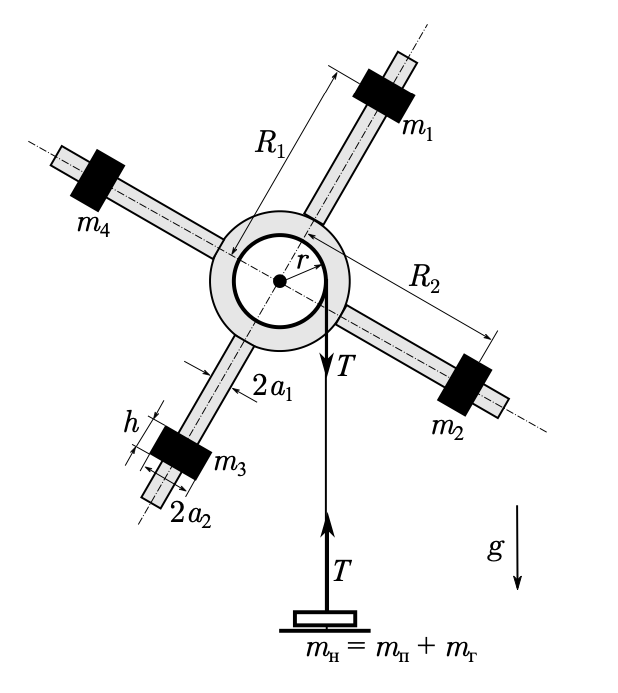
\includegraphics[scale=0.29]{oberbek.png}}
	\caption{Схема установки}
	\label{fig:image}
\end{figure}



\subparagraph*{Вывод уравнения движения маятника: } рассмотрим силы, действующие на маятник. Основной вращающий момент поздаётся подвешенным на нити перегрузком. Непосредственно на маятник действует момент силы натяжения нити: $M_н = rT$, где $r$ -- радиус шкива ($r_1$ или $r_2$). Силу $T$ выразим из уравнения движения платформы $m_н\ddot{y}= m_нg - T$, где $m_н = m_п + m_г$ -- масса платформы с перегрузком. Ускорение платформы связано с угловым ускорением маятника условием нерастяжимости нити $\ddot{y}=\beta r$. Отсюда момент силы натяжения нити 
\begin{equation}\label{2}
M_н = m_нr(g - \beta r).
\end{equation}
Вращению маятника препятствует момент силы трения в оси  $M_{тр}$. Таким образом, с учётом \eqref{2} уравнение  \eqref{1} может быть записано как
\begin{equation}\label{3}
(I + m_нr^2)\beta = m_нgr - {M_{тр}}.
\end{equation}
Заметим, что в наших опытах, как правило, $m_нr^2 \ll I$, и соответственно $M_н \approx m_нgr$, то маятник будет раскручиваться с постоянным угловым ускорением $\beta _0 \approx m_нgr / I$.

Поскольку зависимость момента силы трения от нагрузки на маятник и скорости его вращения не известна (её исследование -- отдельная экспериментальная задача), методика измерения должна быть построена так, чтобы минимизировать или вовсе исключить влияние $M_{тр}$. Можно высказать следующие качественные соображения о природе и величине $M_{тр}$. Она может иметь как составляющую, пропорциональную силе реакции в оси $N$ (сухое трение в подшипниках),  так и составляющую, пропорциональную угловой скорости $\omega$ вращения маятника (вязкое трение в подшипниках и сопротивления воздуха). Учитывая, что сила реакции уравновешенного маятника равна $N = m_мg + T \approx (m_м + m_н)g \approx m_мg $, где $m_м$ -- масса маятника (как правило, $m_м \gg m_н$), можно записать
\begin{equation}\label{4}
M_{тр} \simeq \left(1 + \frac{m_н}{m_м}\right)M_0 + \eta\omega \approx M_0 + \eta\omega,
\end{equation}
где $M_0$ -- момент сил трения для покоящегося маятника при нулевой массе подвеса (минимальное значение силы трения), $\eta$ -- некоторый коэффициент, отвечающий за вязкое трение.

\newpage

\subsection*{Результаты измерений и обработка данных}


Оценим момент сил трения в подшипниках. 
Граничное значение  складывается из массы перегрузка и массы платформы и равно $m_{гр} = 4.80 (г)+ 6.17 (г)= 10.97(г)$. 

Измерения проводились на большом шкифе, радиус которого $r_1 = 1.78(см)$. 

Тогда момент сил трения $M_0 = m_{гр}gr_1 \approx 1.95 \cdot 10^{-3}(Н \cdot м) $.

Проведём измерение коэффициентов прямой $\beta(\omega)$ $k$  и $\beta _0$, чтобы оценить случайную погрешность $\beta _0$.

$$
\begin{tabular}[b]{|c | c | c|}
\hline
	$k$, 1/c & $\beta_0$, рад/$c^2$ & ($\beta_{0сред}$ -$ \beta_{0i})^2, рад^2 / c^4 $ \\ \hline
	$ -0.0078\pm 0.0058$ & $ 0.5126\pm 0,0012 $ & 0.0015 \\
	$ -0.0072\pm 0.0021$ & $ 0.4513\pm 0.0008 $ & 0.005 \\
	$ -0.0079\pm 0.0045$ & $ 0.4388\pm 0.0018$ & 0.0012 \\
	$ -0.0090\pm 0.0017$ & $ 0.4666\pm 0.0085$ & 0.0001\\
	$ -0.0085\pm 0.0070$ &$ 0.4737\pm 0.0016 $ & 0.0001\\
	$ -0.0084\pm 0.0015$ & $ 0.4999\pm  0.0014$  & 0.0007\\
	$ -0,0088\pm 0.0049$ & $ 0.4749\pm 0.0039$ & 0.0001\\ \hline
\end{tabular}
$$

$\beta_{0сред} \approx 0.4740(рад/с^2)$

$\sigma_{случ}= \sqrt{\sum\limits_{i = 1}^{n}\dfrac{(\beta_{0сред} - \beta_{0n})^2}{n(n - 1)}} \approx 0.01 (рад/с^2)$

Проведём измерения коэффициентов прямой $\beta(\omega)$ $k$ и $\beta_0$ при разных массах перегрузка.

$m_0 = 6.17(г)$ -- масса платформы

$r_1 = 1.78(см)$ -- радиус большего шкива

$r_2 = 0.90(cм)$ -- радиус меньшего шкива



$$
\begin{tabular}[b]{| c | c | c | c | c |}
	\hline
	$m_г, г$ & $k, 1/c$& $\beta_0, рад/c^2$ & радиус шкива $r_{1, 2}, см$ & $ M_T, Н \cdot м $ \\ \hline
	68.17 & $-0.0113 \pm 0.0021$ & $ 0.669 \pm0.002 $ & 1.78 & $ 1.21 \cdot 10^{-2}$\\
	106.17 & $ -0.0123\pm 0.0022 $ & $ 1.067\pm 0.007 $ & 1.78  & $ 1.89\cdot 10^{-2}$\\
	146.17  & $ -0.0172\pm 0.0029$ & $ 1.658\pm 0.001$ & 1.78& $ 2.6 \cdot 10^{-2}$ \\
	176.17& $-0.0221 \pm 0.0019$ & $  1.907\pm 0.003$ & 1.78 & $ 3.1\cdot 10^{-2}$\\
	206.17& $ -0.0253\pm 0.0041$ & $ 2.300\pm 0.008$ & 1.78 & $ 3.7\cdot 10^{-2}$\\
	50.37& $ -0.0124\pm 0.0024$ & $0.2275 \pm 0.0090$ &0.90 & $0.45 \cdot 10^{-2}$\\
	106.17& $ -0.0200\pm 0.0076$ & $ 0.6034\pm 0.0048$ &0.90 & $0.96 \cdot 10^{-2}$\\
	146.17& $ -0.0167\pm 0.0024$ & $ 0.8333\pm 0.0032$ &0.90& $ 1.3\cdot 10^{-2}$ \\
	168.17& $ -0.0187\pm 0.0031$ & $ 0.9543\pm 0.0021$ &0.90 & $1.5 \cdot 10^{-2}$\\
	68.17& $ -0.0161\pm 0.0053$ & $ 0.3482\pm 0.0019$ &0.90& $ 0.61\cdot 10^{-2}$ \\ \hline
\end{tabular}
$$
где $M_Т = m_гgr_{1,2}$ -- момент силы натяжения нити

Постороим график $\beta_0(M_т)$ зависимости начального ускорения от момента силы натяжения. Полученная зависимость является прямой пропорциональностью, то есть $\beta_0 = a + bM_Т $.


Коэффициенты $a$ и $b$ вычислим по МНК.

$ a \approx -0.0396  (рад/с^2)$

$b \approx 63.316  (1/{кг \cdot м^2})$

Пересечение с осью абсцисс при $\beta_0 = 0 \Rightarrow M_0 = -a/b\approx 0.63 \cdot 10^{-3}(Н \cdot м)$ -- момент сил трения. (Найденный ранее -- $1.95 \cdot 10^{-3}(Н \cdot м)$). 

Вычислим $I = 1/ b\approx 0.0158(кг \cdot м^2)$. 

Оценим погрешность $I$. Из формулы выше следует, что $\varepsilon_I = \varepsilon_b$.

$\sigma_b = \dfrac{1}{\sqrt{n}}\sqrt{\dfrac{\left\langle \beta_0^2\right\rangle - \left\langle \beta_0\right\rangle^2}{\left\langle \
		M_Т^2\right\rangle - \left\langle М_Т\right\rangle^2} - b^2} \approx 1.74(1/кг\cdot м^2)$ 
	
$\varepsilon_b = \sigma_b / b \approx 0.028$

Тогда $\sigma_I = \varepsilon_I I= \varepsilon_bI \approx 0.005(кг\cdot м^2)$

В итоге имеем:

$$
\boxed{I = (0.0158 \pm 0.0005) кг\cdot м^2}
$$

Проведём измерения зависимости углового ускорения от момента инерции ситемы.



$m_г = 106.17(г)$ -- масса груза
$r = 1.78(см)$ -- радиус шкива

По формуле \eqref{3} имеем:

$$
(I + m_нr^2)\beta = m_нgr - {M_{тр}}
$$

$I \gg m_нr^2 \Rightarrow I_i \approx \dfrac{m_нgr - M_{тр}}{\beta_i}$. 

Полученные значения $I_i$ занесём в таблицу и построим по ним график $I(R^2)$.


$$
\begin{tabular}[b]{| c | c | c | c |}
\hline
$R, см$ &$k, 1/c$ & $\beta, рад/с^2$  & $I, кг\cdot м^2$\\ \hline
17 & $-0.0177 \pm 0.0062$ & $1.004 \pm 0.0015$  & 0.0182\\
15& $-0.1540 \pm 0.0030$ & $ 1.1491\pm 0.0011$  & 0.159\\
13& $-0.0136 \pm 0.0015$ & $ 1.3941\pm 0.0011$ & 0.0131\\
18& $-0.0163\pm 0.0017$ & $0.9090 \pm 0.0023$ & 0.2201\\ \hline
\end{tabular}
$$






Полученные по МНК коэффициенты прямой $I = a + bR^2$ равны:

$a  \approx 0.00564 (кг\cdot м^2)$

$b \approx 0.448 (кг)$

Вычислим $I$ по формуле:
$$
I = I_0 + \sum\limits_{i = 1}^4{(I_i + m_iR_i^2)}
$$
где $I_0$ -- момент инерции системы без грузов, а $I_i = \dfrac{1}{12}m_ih^2 + \dfrac{1}{4}m_i(a_1^2 + a_2^2)$.
Поскольку массы грузов и расстояния до центра масс почти не отличаются $\sum\limits_{i = 1}^4{(I_i + m_iR_i^2)} \approx 4I_1$.
Вычислим эту величину и получим, что $4I_1 \approx7.98 \cdot 10^{-5} (кг\cdot м^2) \ll a \Rightarrow I_0 \approx a$.

Тогда $\sigma_I = \sigma_a = \sqrt{\dfrac{\left\langle I^2 \right\rangle - {\left\langle I \right\rangle}^2 - b^2\left(\left\langle {R^4} \right\rangle - {\left\langle {R^2 }\right\rangle}^2\right)}{n}} \approx 0.00002 (кг\cdot м^2)$

Имеем 
$$
\boxed{I_0 = (0.00564 \pm 0.00002) (кг\cdot м^2)}
$$


Найдём $I_0  $ другим способм. Измерим $k$  и $\beta_0$  при перегрузке массой $m_п = 106.17(г)$ без грузов на маятнике.Полученные данные занесём в таблицу.

$$
\begin{tabular}[b]{| c | c |}
\hline
$k, 1/c$ & $\beta_0, (рад/ с^2)$ \\ \hline
$-0.0 452 \pm 0.0031$ & $ 3.238\pm0.006 $ \\
$-0.0407 \pm0.0056 $ & $ 3.189\pm0.009 $ \\
$-0.0839 \pm 0.001$ & $ 3.776\pm0.002$ \\ \hline
\end{tabular}
$$

$\left\langle \beta_0\right\rangle = 3.401(рад/ с^2)$

$I_0 \approx \dfrac{m_пgr - M_0}{\beta_0} \approx0.00537 (кг\cdot м^2)$

 \begin{tabular}{c}
	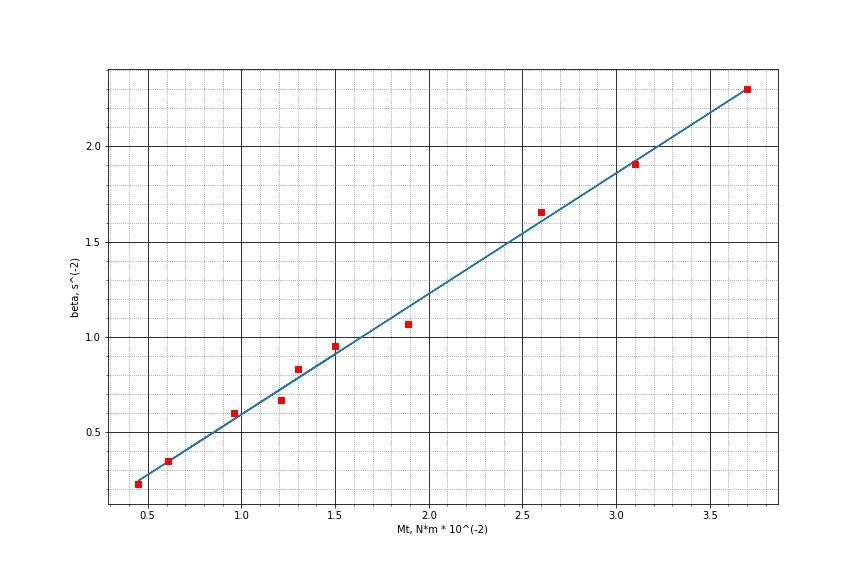
\includegraphics[scale=0.45]{g1.jpg} \\
	График зависимости $\beta_0 = a + b M_т$
\end{tabular}

\begin{tabular}{c}
	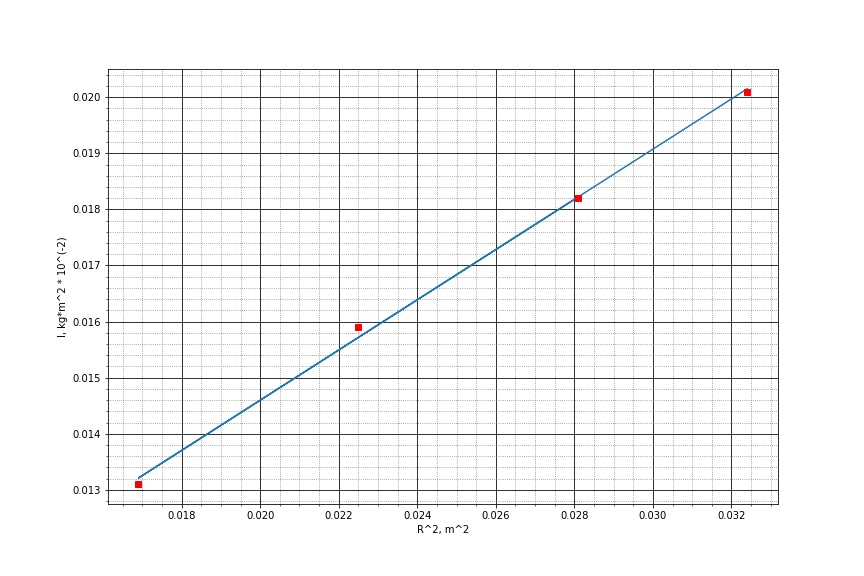
\includegraphics[scale=0.45]{g2.jpg} \\
	График зависимости $I = a + bR^2$ 
\end{tabular}


\newpage

\subsection*{Вывод}

Мы убедились, что угловое ускорение маятника обратно пропорционально моменту инерции тела и прямо пропорционально моменту прикладываемых сил. Помимо этого было выяснено, какой вклад в общий момент сил вносит момент силы трения в оси вращения.





\end{document}
